\chapter{Motivation}

\section{Science as an incremental, open process}

The history of science is all too often taught as a chronological list of discoveries. There is undeniable value in this approach as it reflects the arrow of complexity of notions. However, it leads to a very simplified image of the development of scientific knowledge: one big idea bringing over the next and so on. On page~\pageref{table:historyDiff}, I too show the history of diffraction as a table of chronological events. These are big shift events, which radically and permanently changed the way future science was to be done in this area. A good number of names in this table were awarded for their significant contribution with Nobel prizes. Nevertheless, the table is clearly a gross simplification of history, omitting, due to lack of space, the incremental refinement and maintenance work that supported and propelled the bigger ideas. It is quite common for important work of individual voices to be wiped away from science history as we associate a breakthrough to a single name or even to a small group of people. Seeing the bigger picture is, undeniably, worthwhile, but we must not mistake it for the full picture.

The ``unremarkable'' work done by the rest of the community, not awarded prestigious prizes, is not less important for the advancement of science. Quite the opposite. Neither science nor culture truly advance in big steps. In a recent study published in Nature, Miu \etal~\cite{Miu2018} looked at the way pieces of software get improved by a community of developers in a simulation of cumulative culture evolution. One of the observations was that the vast majority of advances are of an incremental type and not, as the scientific community expect, leaps in knowledge. Observing the strong positive breakthrough bias of scientific publishing, one would find it hard to assume that enough credit is given to the ``tweakers''. 

Another critical observation was that big changes in the paradigm are more likely to turn out unsuccessful than smaller tweaks. Remember the Nobel prize in medicine awarded for the ``discovery'' of brain lobotomies\footnote{``for his discovery of the therapeutic value of leucotomy in certain psychoses''-- The Nobel Prize in Physiology or Medicine 1949~\cite{Nobel49}.}? Thankfully, neuroscience moved away from this particular scientific breakthrough. And it did that with small, incremental improvements on the understanding of the brain. Any sort of conversation about the development of science focused only on the leaps of knowledge must ultimately be misrepresenting the scientific process.


In this paradigm of scientific value misrepresentation, scientific code suffers perhaps even more. The philosopher Daniel C. Dennett, in his latest book \textit{From bacteria to Bach and back}~\cite{Dennett} makes the case that evolution is not only a good protocol for developing fit biological organisms but can, in fact, be successfully applied to a variety of concepts, perhaps, he argues, consciousness, the human mind and even code development. The latter analogy I find compelling. Similarly to adaptable organism having emerged from surviving a variety of conditions, the power of good code stands in the number of iterations it went through. Of course, we cannot wait around for functional code to ``occur'' as the results of tens of millions of years of iterations, and, after all, we expect developers to be somewhat wiser than the random processes occurring in nature. Nevertheless, in the end, each iterative step has the chance to rectify errors or limitations in the code, weed out unnecessary/old lines and replace them with new, more optimised, features. Established software tends to be software reviewed by many pairs of eyes. Yet, scientific software continues to be developed and  maintained by small groups and destined to see the light of only a handful of iterations.  


To add insult to injury, scientific code is rarely developed to be open and even more rarely made easily accessible. Here is another anecdotal evidence of why I think this a counter-intuitive way of following the scientific method. Two condensed matter groups set out, independently, to predict the behaviour of supercooled water, and, even though they implemented the same method, their results contradicted each other for seven straight years~\cite{supercool}. During this time, while the groups were in contact to one another, the actual lines of code never changed hands. When it finally did, a bug was discovered by the ``competin'' team in just a few months. I'm pointing out that we could have known in a few months, not seven long years, that water is predicted to change phase when supercooled. When scientific groups working in the same field do not collaborate with each other for whatever reason, it is science that suffers.


In the light of all these, I want my thesis work to make a positive tweak in the endeavour of making electron diffraction in the SEM a well-understood phenomena in the electron microscopy community. I aim for this work to aid the understanding of why we can observe and how we can study dislocations in the SEM and I do not expect it to be the definitive attempt. For these reasons I tried to make this document as accessible as possible for whoever wants to continue on this journey. I tried to explain in depth the building blocks I used and why I chose them, I provide access to whatever code I ran or wrote and I offer a small collection of extra materials. May your code and science be even a little bit better than mine!



\section{Implementations}

I will refer throughout this document to supplementary pieces of code, most in \emph{Python} and some in \emph{Fortran95}. I will try to describe in detail what they do, sometimes I will include pseudocode and other times I will just state the relevant equations. They can all be found on my, otherwise rather pristine, public GitHub repository~\cite{myGitHub}. 

The Python scripts have been written in Python 2 which can be easily installed on Ubuntu machines from the package manager or by typing in 18.04 or later:
\begin{verbatim}
$ apt install python-minimal
\end{verbatim}
Files containing Python script can be easily recognised from the \textit{.py} file type and can be ran with with:
\begin{verbatim}
$ python filename.py
\end{verbatim}

To run Fortran code on a Ubuntu machine use the gfortran compiler, which again can be found in the package manager or can be installed via:
\begin{verbatim}
$ apt install gfortran
\end{verbatim}

For the smaller scripts I use \href{http://jupyter.org}{\texttt{Jupyter}}~\cite{Jupyter} notebooks written in Python. I will assume the reader has Python 2.7 or greater installed. The \href{https://anaconda.org/}{\texttt{Anaconda}} Python distribution~\cite{Conda} ships with Jupyter among other packages useful for scientific computation. However, if you have Python already installed then you can use the package manager \href{https://pypi.org/project/pip/}{\texttt{pip}} to add new libraries:
\begin{verbatim}
$ pip install jupyter
\end{verbatim}
To start a Jupyter notebook kernel you just type:
\begin{verbatim}
$ jupyter notebook
\end{verbatim}
And navigate to the desired script file. Individual cells are compiled with \texttt{Shift} + \texttt{Enter}.

In some notebooks I use the \href{https://plot.ly/}{\texttt{plotly}} package ~\cite{Plotly} for plotting. These figures are interactive but do require an account on the \href{https://plot.ly/}{\texttt{plotly} website}\footnote{ \texttt{Plotly} website url is \href{https://plot.ly/}{https://plot.ly/}.}.  

\section{Diffraction and the SEM}


The Venn diagram of electron diffraction and scanning electron microscopy (SEM) (Fig.~\ref{Fig:Venn}) is not showing a very small overlap. Diffraction in general, and particularly that of electrons, which  we will discuss in more details in Chapter~\ref{Chap:Diffraction} on page~\pageref{Chap:Diffraction} is a mature and well understood subject. So is the now ubiquitous materials investigation tool that is the SEM, which we will briefly cover on page~\pageref{sec:sem}. 

The group of people studying both these fields is a very select one. The techniques based on electrons diffraction in the SEM either do not have a dedicated conference such as the \textit{channelling} family; this includes electron channelling patterns (ECPs) and electron channelling contrast imaging (ECCI), and we will explore in Chapter~\ref{chap:ECCI} on page~\pageref{chap:ECCI}, or do have dedicated conferences; this is the case for the backscattered/fore-scattered diffraction family which includes electron backscattered diffraction (EBSD) and, more recently, transmission Kikuchi diffraction (TKD), which will be described in Chapter~\ref{chap:TKD} on page~\pageref{chap:TKD}, but are dominated by material scientists interested more in understating the materials rather than the physics of the characterisation technique. 

\begin{figure}[ht]
\centering
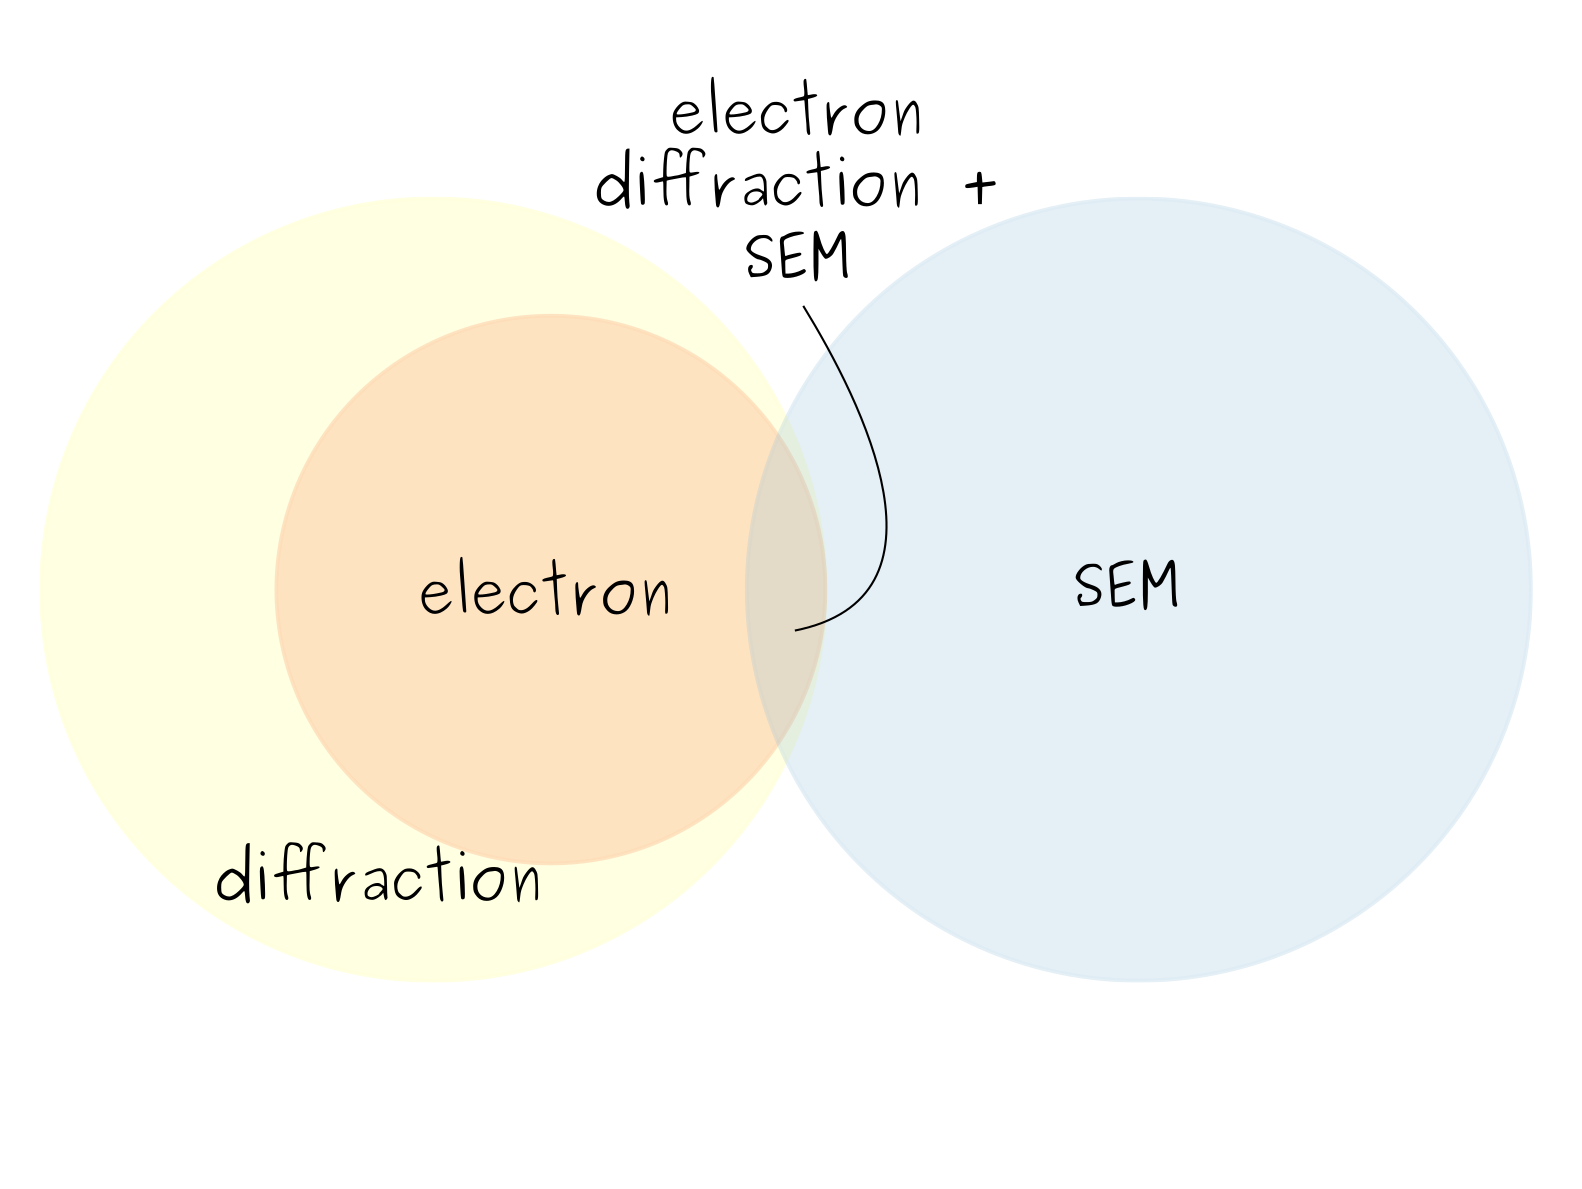
\includegraphics[width=0.72\linewidth]{Figures/VenSEM.png}
\caption[SEM and electron diffraction Venn diagram.]{The Venn diagram of diffraction (yellow), electron diffraction (orange) and SEM (blue), based on number of results in Google Scholar, makes up the subject of this thesis.}
\label{Fig:Venn}
\end{figure}

Some of these techniques are more novel than the others, but all of them carry mysteries about aspects of the underlying physical processes. These unanswered questions are enticing not only from the aspect of fundamental physics, but also as a promise of more information that could be derived from these measurements.





\subsection{Diffraction}

Starting with page~\pageref{Chap:Diffraction} I will spend an entire chapter on the powerful characterisation technique that is diffraction. There are only handful more elegant ideas out there then the power of observing the reciprocal space of an ordered arrangement of atoms, taking us very quickly to the conundrum of why is maths such a good description of reality.  But let us not digress. 

The geometry of diffraction is beautifully simple in the form of Bragg's law. Perhaps less intuitive is the fact that Bragg's law being satisfied is not a guarantee of non-zero diffracted intensity. This behaviour is going to depend not only on the crystal system as Bragg law does, but instead it is going to be a map of the space group symmetry of the material under investigation. 

It is important to understand the basic diffraction behaviour in a material system before trying to derive information from a diffraction based technique applied on that material system. I will show, in Chapter~\ref{Chap:Diffraction}, theoretical predictions for electron diffraction relating parameters, such as scattering and structure factor for a few group-III nitride materials: AlN, GaN and InN. 

While all particles diffract in the same way, electrons interact more strongly with matter and simplifications that could be done in the more established case of X-rays diffraction predictions and not acceptable when it comes to electrons. In the rest of that chapter I will review the dynamical model of electron diffraction and show how it incorporates the diffraction parameters mentioned above.

Because we cannot talk about diffraction without some solid knowledge of crystallography, I cover extensively the basics of crystallography and crystallographic computations in Chapter~\ref{chap:Background}. Since diffraction is the map of the crystal symmetry I examine in Appendix~\ref{Chap:Symmetry} on page~\pageref{Chap:Symmetry} the full $\mathbf{P6_3mc}$ symmetry of the wurtzite system.  

\subsection{The scanning electron microscope}
\label{sec:sem}
% microscopy
The phenomena described in the previous section occur at a scale too small to be measured by the naked eye. Luckily,  development of science had brought us two main extension  to the range of scales we can study. On one hand,  the telescope brings very distant object closer and is optimised to collect as much light as possible and, on the other, the microscope makes very close objects appear many times larger.
Interestingly, both these aids can be traced back to a \nth{17} century event: the development of glass lenses used in spectacles. Fundamentally, both these visual extensions are governed by the same optics laws. 

While modern light microscopes can showcase a magnification of about $2000\times$, their spatial resolution is limited by the wavelength of visible light, which is of the order of hundreds of nanometers, through Abbe's equation. One way around it is to use  different imaging particles, for instance, X-rays or electrons which have significantly smaller wavelengths (see Table~\ref{table:diffractingParticles} for wavelength comparison between X-ray photons and electrons).   

We will explore further the electron microscope, excellent detailed description of which can be found in ref.~\cite{Hearle72} and ref.~\cite{Reimer13}. There are various ways of generating an electron beam. For instance, in our (old FEI now Thermo Fisher ) SEM, a wire of tungsten with a sharp tip is used to generate a beam of electrons through field emission. This beam is then focused through a series of condenser lenses onto the surface of a sample such that the beam spot size on the sample can go down to  \SI{1}{\nano \meter} in diameter in practice.  After the beam is focused on the sample, scanning coils are used to deflect the beam on a set of orthogonal directions in a predefined manner. 

Depending on the geometry of imaging\footnote{ But also electron beam energy and sample preparation procedure.} we classify electron microscopy into \textit{transmission electron microscopy} (TEM) on one hand, where the image is formed by electrons which have travelled through a very thin sample, and \textit{scanning electron microscopy} (SEM), where the imaging electrons come from the same, top surface of the sample with which the incident beam interacts with\footnote{ Advances in both worlds make this distinction imperfect. There is an exception to the rule above, in the form of transmission SEM. To make things even harder to classify there is also scanning TEM.}. Both of them have advantages and disadvantages. The TEM geometry minimises the lateral spread of the electron-sample interaction volume providing therefore higher spatial resolution, but it also limits its field of view. Additionally, thinning the sample to the sizes required by this geometry can be cumbersome, time consuming and irremediably damaging to the sample. There is also the additional question the microscopist must answer, whether the features observed are intrinsic to the sample or were introduced during the polishing process. On the other hand, the SEM requires minimal sample preparation since the thickness of the sample does not limit its capabilities. The downside, as we will see, is that the SEM is not optimised for diffraction contrast in the same way the TEM is. 


Since electrons interact strongly with matter they can generate a plethora of signals for one to measure in the SEM using the right, specialised detector:
\begin{itemize}
    \item Most commonly, low-energy ($<$\SI{50}{\electronvolt}) \textit{secondary} electrons (SE) are ejected by those atoms with which the primary beam electrons have inelastically scattered. With such low energies these electron cannot come from very deep in the sample, which means the interaction volume is narrow enough to provide a tool for high resolution surface imaging. These electrons are collected by attracting them to an electrically biased grid and then further accelerated towards a phosphor or scintillator, in what is know as a Everhart-Thornley detector~\cite{ETdetector}.
    
    
    
    \item In addition to secondary electrons, excited atoms will also emit a variety of electromagnetic radiation such as characteristic X-rays which can provide information on the distribution of different elements in the sample as long as the SEM is equipped with wavelength dispersive \textit{X-ray spectrometers} (WDS) or energy-dispersive X-ray spectroscopy (EDS). 
    
    \item As the atoms relax back to their ground state after the encounter with the high energy electrons, they can generate light which can provide useful optical information in a technique known as \textit{cathodoluminescence} (CL)~\cite{Paul11}.
    
    \item The primary beams electrons will too escape the sample, after having lost more or less energy through inelastic scattering. This implies, that, at some point in their trajectory, the incident electrons suffered a large angle elastic scattering such that they turned back to the surface of entry. All the incident electrons that suffer an elastic scattering event and manage to escape through the entry surface are collectively known as \textit{backscattered electrons} (BSE) and can be detected by a scintillator or a solid state detector. Since heavier atoms will elastically scatter electrons more strongly, BSEs are used to detect contrast due different chemical compositions. Additionally, if the detector is not collecting a symmetric radial distribution of BSEs, then the image will also contain strong topographic contrast. 
    
 \begin{figure}[ht]
\centering
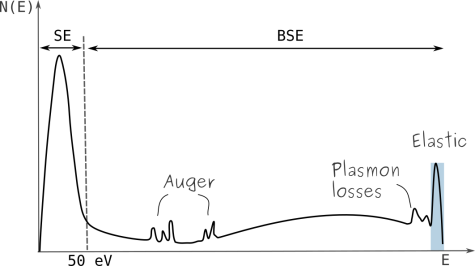
\includegraphics[width=0.62\linewidth]{Figures/spectrum.png}
\caption[SEM electrons energy spectrum.]{Schematic energy spectrum of secondary and backscattered electrons in an SEM [after~\cite{bell12}].}
\label{Fig:Espectrum}
\end{figure}

    \item Figure~\ref{Fig:Espectrum} shows the energy distribution of electrons reaching the BSE detector for an incident beam of energy $E$. Over-imposed on the BSE energy curve are a few other signals but we will only talk here about the elastic peak as it makes the core of this work. A subset of BSEs will loose almost no energy before reaching the detector, either because they have been backscattered by the top layer of the sample, or, more likely, because they underwent diffraction, a case in which inelastic scattering processes are reduced (see the discussion on channelling on page~\ref{sec:channelling}). We will call this the \textit{elastically BSE}. This signal can provide information on the crystallographic orientation of a small region of the sample or about small changes in local strain. More on this in the rest of the thesis. One could use energy sensitive detectors to select only this signal~\cite{Stefano}.
\end{itemize}




We will be concerned in this document only with elastically scattered BSEs (in Chapter~\ref{chap:TKD} we will also talk about forward scattered electrons (FSE)). The sample geometry optimised for this signal is shown below in Fig.~\ref{Fig:sillySEM}. The sample is tilted with respect to the incident beam and the detector is positioned such that it can collect the solid angle of the backscattered electrons that provides the highest intensity. We call this geometry forward-scattering. 



\vspace{0.2cm}

\noindent\begin{minipage}{0.5\textwidth}
The method of operation of the SEM is shown Figure~\ref{Fig:sillySEM}. A collimated beam of electrons is focused on the surface of a tilted sample. The beam is then scanned in a raster manner over the area of interest on the sample. The detector collects one pixel worth of BSEs intensity at a time. The beam is moved by the deflector coil to the next position on the sample defined by the step size. The resulting image is made up of the ordered collected pixels, and, at the end of the scan, has as many pixels as steps used in scanning.  
\end{minipage}%
\begin{minipage}{0.5\textwidth}
    \centering
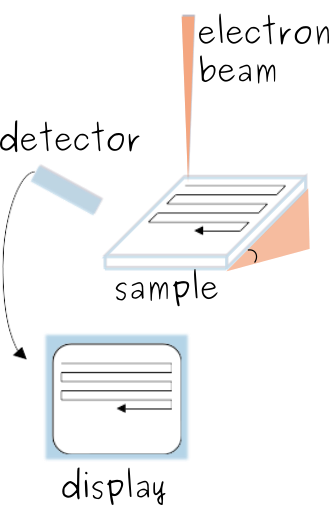
\includegraphics[width=0.48\linewidth]{Figures/sillySEM.png}
\captionsetup{width=.7\linewidth}
\captionof{figure}{SEM schematics in forward-scattering geometry.}
\label{Fig:sillySEM}
\end{minipage}

\vspace{0.4cm}



% TILT
The tilt of the sample in the forward-scattered geometry in the SEM ensures that  enough electrons reach the detector. It also makes the geometry of diffraction very different from that in the TEM. The sample's z-direction in the SEM is not the same as the beam direction which is the case for the TEM sample geometry. This means that if we are to use the diffraction models developed for TEM, they must be generalised for the sample tilt.  More about this in the next chapter. 

References~\cite{Hearle72, Reimer13} discuss the electron optics as well and we will not delve on it here. We will however mention that the tilt of the sample affects the ``squareness'' of the scanned area. The trapezoidal area scanned will produce a distorted image, which can be corrected to some degree using the tilt correction function (see page 50 in ref.~\cite{SEMbooklet} for tilt correction artefacts). The tilt can also change the shape of the beam on the sample which not only affects the imaging but also the diffraction interaction volume. 


%relativistic correction
Let us shortly address relativistic corrections for electrons used in electron microscopy. The de Broglie equation for the relativistic electron  wavelength, $\lambda$, can be written in terms of the accelerating voltage $V$ (equation 2.4 in \cite{goodhew88}) as:
\begin{equation}
    \lambda = \sqrt{\frac{150}{V + 10^{-6}\, V^2}} \,\, [\si{\angstrom}]
\end{equation}
where the second term is the correction term and becomes important for voltages greater than $20$ \si{\kilo \electronvolt} as we can see in Table~\ref{Table:wavelength}. For SEM applications discussed in this work we will focus on $20$ \si{\kilo \electronvolt} incident electrons, and discard, quite acceptably, relativistic effects. 

\begin{table}[ht]
\caption{Corrected and uncorrected electron wavelengths for voltages used in  electron microscopy.}
\label{Table:wavelength}
\vspace{-0.4cm}
\centering
\begin{longtable}{l c c c}\toprule
             \multirow{2}{*}{\tabhead{Voltage [\si{\kilo \electronvolt}] }} &  \multirow{2}{*}{\tabhead{Lorentz factor $\gamma$} \hspace{0.4cm}}  & \multicolumn{2}{c}{\tabhead{Wavelength  $\lambda$ [\si{\angstrom}]}}\\ \cmidrule{3-4}
              &  &\tabhead{Uncorrected}        &  \tabhead{Corrected}  \\ \midrule
20   & 1.04  & 0.086 & 0.086  \\
100  & 1.20  & 0.039 & 0.037  \\
1000 & 2.93  & 0.012 & 0.009  \\
\bottomrule
\end{longtable}
\end{table}


